\documentclass[12pt]{article}
\usepackage[cm]{fullpage}
\usepackage[usenames,dvipsnames]{color}
\usepackage{sectsty}
\usepackage{listings}
\usepackage{color}
\usepackage{textpos}
\usepackage[usenames,dvipsnames,table]{xcolor}
\usepackage[small, bf]{caption}
\usepackage{amssymb,latexsym}
\usepackage{amsmath}
\usepackage{xltxtra,xunicode,xgreek}
\usepackage[colorlinks=true, linkcolor = blue, citecolor=blue]{hyperref}
\usepackage[ddmmyyyy]{datetime}
\usepackage{multirow}
\usepackage{tikz}
\usepackage{qtree}
\usepackage{float}
\usepackage{minted}
\usepackage[boxed]{algorithm2e}
\usepackage{textcomp}
\usepackage{fullpage} 
\usepackage{url} 
\usepackage{doc}
\usepackage{xcolor}
\usepackage{tabu}
\usepackage{colortbl}
\usepackage{float}


\definecolor{lightgray}{gray}{0.98}
\setmainfont[Mapping=tex-text]{CMU Concrete}
\setmonofont{Courier New}
\newcommand{\tab}{\hspace*{2em}}
\newcommand{\rom}[1]{\uppercase\expandafter{\romannumeral #1\relax}}
\setlength{\parindent}{0pt}
\renewcommand\listingscaption{Κώδικας}

\usemintedstyle{tango}
\SetKw{Kwdto}{downto}

\begin{document}
\begin{titlepage}
\begin{center}


\includegraphics[scale=0.15]{pyrforos.pdf}\\
ΕΘΝΙΚΟ ΜΕΤΣΟΒΙΟ ΠΟΛΥΤΕΧΝΕΙΟ \\
ΣΧΟΛΗ ΗΛΕΚΤΡΟΛΟΓΩΝ ΜΗΧΑΝΙΚΩΝ KΑΙ ΜΗΧΑΝΙΚΩΝ ΥΠΟΛΟΓΙΣΤΩΝ \\ 
\vspace{0.5em}

\medskip 

\def\doubleline{

    \vspace{0.1em}
    \line(1,0){530}\

    \vspace{-1.5em}
    \line(1,0){530}

}
\doubleline
\vspace{1.3em}

{\large \textbf{Τεχνητή Νοημοσύνη}\\
 \medskip
7ο εξάμηνο, Ακαδημαϊκή περίοδος 2012-2013 \\ \bigskip \medskip}

\vspace{1.5em}
{\LARGE \textbf{Άσκηση 1\\}}
\vspace{32em}

\begin{tabular}{l l}
Νίκος Γιανναράκης & 03108054 \\
Ζωή Παρασκευοπούλου & 03108152 \\
\end{tabular}\\
\bigskip
\today
\end{center}
\end{titlepage}
\tableofcontents

\pagebreak

\section{Περιγραφή Προβλήματος}
Σκοπός της άσκησης είναι ο σχεδιασμός και η υλοποίηση αλγορίθμου για ένα robot (1) που θα του επιτρέψει να συναντήσει ένα άλλο robot (2) το οποίο κινείται με τυχαίο τρόπο στο χώρο. Πιο συγκεκριμένα, δίνονται οι αρχικές θέσεις των δύο robot και ένας χάρτης που περιγράφει το χώρο και τα εμπόδια σε αυτόν (σημεία του χώρου που τα δύο robot δε μπορούν να βρεθούν). Το robot (1) γνωρίζει πάντα τη θέση του robot (2), έτσι μετά από κάθε (τυχαία) κίνηση του robot (2), το robot(1) χρησιμοποιεί τον αλγόριθμο που σχεδιάσαμε έτσι ώστε να πλησιάσει στο robot (2). Η συνάντηση των δύο robot εφόσον ο χάρτης του χώρου το επιτρέπει, είναι εγγυημένη από το γεγονός ότι το robot (1) κινείται με τριπλάσια ταχύτητα από το robot (2) , δηλαδή για κάθε κίνηση του robot (2) αυτό μπορεί να πραγματοποιήσει τρεις κινήσεις. Και τα δύο robot κινούνται μόνο προς τα μπροστά, πίσω, αριστερά ή δεξιά, όχι διαγώνια.
\section{Επίλυση προβλήματος}
Για την επίλυση του προβλήματος χρησιμοποιήσαμε τη γλώσσα προγραμματισμού Haskell.
\subsection{Δομές δεδομένων}
Η υλοποίηση μας χρησιμοποιεί αμιγώς συναρτησιακές δομές δεδομένων, κατά κύριο λόγο Sets και Maps. Ορίσαμε επίσης δύο βασικούς τύπους, τον τύπο \textbf{Point} που αναπαριστά ένα σημείο στο χώρο με βάση τις συντεταγμένες του και τον τύπο Robot που αναπαριστά ένα Robot με βάση τη θέση του στο χώρο και την ταχύτητα με την οποία κινείται σε αυτόν (το πεδίο της ταχύτητας δε χρησιμοποιήθηκε στην υλοποίηση μας). Δίνονται οι ορισμοί των δύο τύπων:
\begin{minted}{haskell}
data Point = Point { x :: Int,
                     y :: Int }
    deriving (Show, Ord, Eq)
\end{minted}

\begin{minted}{haskell}
data Robot = Robot { position :: Point,
                     velocity :: Int }
    deriving (Show, Ord, Eq)
\end{minted}
\subsubsection{Μοντελοποίηση χώρου κίνησης}
Για την αναπαράσταση στη μνήμη του χώρου στον οποίο κινούνται τα δύο robot χρησιμοποιήσαμε μία δομή Map (key => val) όπου ως key χρησιμοποιήσαμε ένα σημείο του χώρου ορισμένο από τον τύπο \textbf{Point} και ως value την τιμή που διαβάστηκε από το αρχείο εισόδου, `Χ` για κάποιο εμπόδιο στο συγκεκριμένο σημείο ή `Ο` όταν το σημείο είναι προσβάσιμο. 
\subsubsection{Μοντελοποίηση του χώρου καταστάσεων}
Για την αναπαράσταση στη μνήμη του δέντρου αναζήτησης ορίσαμε μία παραμετρική δομή με όνομα \textbf{AStar}. Ο ορισμός της δομής δίνεται παρακάτω:
\begin{minted}{haskell}
data AStar node cost = AStar { visited   :: !(Set node),
                               openSet   :: !(PSQ node cost),
                               distance  :: !(Map node cost),
                               heuristic :: !(Map node cost),
                               ancestor  :: !(Map node node),
                               final     :: !(Maybe node) }
    deriving Show
\end{minted}
Η δομή αυτή αναπαριστά μία κατάσταση στην οποία έχει επέλθει ένα robot (στη συγκεκριμένη περίπτωση). Μεταξύ άλλων μέσα στη δομή υπάρχουν αποθηκευμένοι οι κόμβοι που ακολούθησε το robot μέχρι να φτάσει στη θέση-στόχο (πεδίο ancestor) και αν όντως βρίσκεται στη θέση-στόχο ή δε τα κατάφερε να φτάσει ποτέ (πεδίο final). Τα υπόλοιπα πεδία αφορούν τις πληροφορίες που απαιτεί ο αλγόριθμος A* που χρησιμοποιήθηκε για την αναζήτηση.
\subsection{Βασικές συναρτήσεις}
\subsubsection{aStar}
Για την υλοποίηση του A* ορίσαμε τη συνάρτηση \textbf{aStar} ως εξής:
\begin{minted}{haskell}
aStar :: (Ord a, Ord c, Num c) =>
         (a -> Set a)     
         -> (a -> a -> c) 
         -> (a -> c)      
         -> (a -> Bool)  
         -> a             
         -> (Maybe [a], Int)  
\end{minted}
Όπως προκύπτει και από τον ορισμό της η συνάρτηση \textbf{aStar} παίρνει τα εξής ορίσματα:
\begin{enumerate}
\item Mία συνάρτηση που βρίσκει όλα τα πιθανά παιδιά στο δέντρο αναζήτησης (στη δική μας περίπτωση όλες τις πιθανές κινήσεις που μπορεί να κάνει το robot) μίας κατάστασης τύπου a. Η συνάρτηση αυτή παίρνει ως όρισμα μία κατάσταση με τύπο a και επιστρέφει ένα Set από στοιχεία τύπου a.
\item Μία συνάρτηση που υπολογίζει την πραγματική απόσταση μεταξύ δύο γειτονικών καταστάσεων (στην περίπτωση μας η απόσταση μεταξύ του γονέα και του παιδιού είναι πάντα 1 εφόσον το παιδί έχει κάνει μία κίνηση προς μία από τις 4 δυνατές κατευθύνσεις). Η συνάρτηση αυτή παίρνει ως όρισμα δύο γειτονικές καταστάσεις και επιστρέφει το κόστος μετάβασης από την πρώτη στη δεύτερη.
\item Μία ευρεστική συνάρτηση  υπολογισμού του κόστους μετάβασης από την τωρινή κατάσταση στην κατάσταση στόχο, η συνάρτηση αυτή δέχεται ως όρισμα μία κατάσταση τύπου a και επιστρέφει το εκτιμώμενο κόστος μετάβασης τύπου c.
\item Μία συνάρτηση που δέχεται ως όρισμα μία κατάσταση τύπου a και αποφασίζει αν αυτή είναι η κατάσταση στόχος ή όχι. Επιστρέφει bool.
\item Μία αρχική κατάσταση τύπου a από την οποία ξεκινάει η αναζήτηση.
\end{enumerate}
Η συνάρτηση \textbf{aStar} επιστρέφει μία τούπλα με τύπο (Maybe [a], Int). Το πρώτο όρισμα της τούπλας είναι μία λίστα από καταστάσεις σε περίπτωση που βρέθηκε η κατάσταση στόχος ή ένα Nothing σε περίπτωση που η αναζήτηση απέτυχε. Το δεύτερο όρισμα της τούπλας είναι ένας ακέραιος που δείχνει πόσοι κόμβοι του δέντρου αναζήτησης εξετάστηκαν. 
Επίσης από τον ορισμό της συνάρτησης προκύπτει ότι ο τύπος a (τύπος της κατάστασης) θα πρέπει να επιδέχεται διάταξη, όπως επίσης και ο τύπος c (τύπος κόστους μετάβασης) που θα πρέπει επιπλέον να είναι και κάποιος αριθμητικός τύπος.
Στην περίπτωση μας το a είναι ο τύπος Robot (ο οποίος εξ ορισμού κληρονομεί την κλάση τύπων Ord) που ορίσαμε παραπάνω και το c ο τύπος Int.
\subsubsection{traverse}
Ορίσαμε επίσης τη συνάρτηση \textbf{traverse} η οποία καλείται από τη συνάρτηση \textbf{aStar} και στην ουσία πραγματοποιεί την αναζήτηση στο χώρο καταστάσεων.
Oρισμός της συνάρτησης \textbf{traverse}: 
\begin{listing}[H]
\begin{minted}[bgcolor=lightgray]{haskell}
traverse :: (Ord n, Ord c, Num c) =>
         (n -> Set n)     -- function returning neighbours of a node
         -> (n -> n -> c) -- distance function
         -> (n -> c)      -- heuristic function
         -> (n -> Bool)   -- is final?
         -> n             -- root node
         -> AStar n c     -- final state
\end{minted}
\caption{Oρισμός της συνάρτησης \textbf{traverse}}
\end{listing}

Η \textbf{traverse} παίρνει τα ίδια ορίσματα με την \textbf{aStar} και επιστρέφει μία κατάσταση τύπου AStar n c. Στη δική μας περίπτωση τύπου AStar Robot Int. Η κατάσταση αυτή είναι η τελική κατάσταση της αναζήτησης, μέσα από αυτή μπορούμε να βρούμε όλες τις ενδιάμεσες θέσεις του robot καθώς είναι αποθηκευμένες στο πεδίο ancestor.
\subsubsection{Ευρεστικές συναρτήσεις}

Υλοποιήσαμε έναν υπο-εκτιμητή μέσω της απόστασης Manhattan
$$d(p,q) = \Vert p - q \Vert_1 = \sum_{i=1}^{n} \vert p_i - q_i \vert$$
\begin{listing}[H]
\begin{minted}[bgcolor=lightgray]{haskell}
manhattanNorm ::  Point -> Point -> Int
\end{minted}
\caption{Ορισμός του υπο-εκτιμητή με χρήση της Manhattan απόστασης}
\end{listing}
Υλοποιήσαμε έναν υπερ-εκτιμητή με βάση την ευκλείδεια απόσταση
$$d(p,q) = \Vert p - q \Vert_2 = (p_n-q_n)^2 = \sqrt{\sum_{i=1}^{n} (p_i-q_i)^2}$$
\begin{listing}[H]
\begin{minted}[bgcolor=lightgray]{haskell}
euclideanNorm ::  Integral b => Point -> Point -> b
\end{minted}
\caption{Ορισμός του υπερ-εκτιμητή με χρήση της Ευκλείδειας απόστασης στρογγυλοποιημένης προς τα κάτω}
\end{listing}
Και οι δύο συναρτήσεις παίρνουν ως όρισμα δύο σημεία του χώρου, όπως τα ορίσαμε με βάση τον τύπο Point και επιστρέφουν έναν ακέραιο.
\section{Στατιστικά αποτελέσματα}
Σε αυτή την ενότητα παραθέτουμε γραφήματα που αναπαριστούν το συνολικό χρόνο εκτέλεσης συναρτήσει των καταστάσεων που παράχθηκαν κατά τη διαδικασία αναζήτησης. Για την παραγωγή των στατιστικών αποτελεσμάτων χρησιμοποιήσαμε 6 test-cases διαφορετικού μεγέθους. Οι δοκιμές έγιναν και με τη χρήση υπο-εκτιμητή (admissible heuristic) και με τη χρήση υπερ-εκτιμητή  (non-admissible heuristic).

\begin{figure}[H]
\taburowcolors[2]{white .. black!20}
\sffamily\footnotesize
\tabulinesep=6pt
\begin{tabu}{|>{\cellcolor{black!80}\color{white}}c|X[cm]|X[cm]|X[cm]|}
\hline
\rowcolor{black!80}\strut \color{white}Testcase & \color{white}Grid 1 & \color{white}Robot 1 & \color{white} Robot 2 \\
test1  &  (99, 50)  &  (15, 2) & (84, 89) \\
test2  &  (99, 200) & (1, 1) & (99, 200) \\
test3  &  (168, 60) & (4, 20) & (160, 40) \\
test4  &  (99, 100) & (3, 11) & (80, 95) \\
test5  &  (99, 100) & (1, 1) & (89, 95) \\
test6  &  (180, 180) & (4, 1) & ( 180, 179) \\
\hline
\end{tabu}
\caption{Παράμετροι testcase}
\end{figure}

\subsection{Admissible heuristic}
\begin{figure}[H]
\taburowcolors[2]{white .. black!20}
\sffamily\footnotesize
\tabulinesep=6pt
\begin{tabu}{|>{\cellcolor{black!80}\color{white}}c|X[cm]|X[cm]|}
\hline
\rowcolor{black!80}\strut \color{white}Testcase & \color{white}States & \color{white}Time \\
test1  &  31019  & 0.3735411 \\
test2  &  668160 & 9.4400402 \\
test3  &  741269 & 0.9625383 \\
test4  &  90544  & 1.2119474 \\
test5  &  131380 & 1.6911385 \\
test6  &  402761	& 5.683861 \\
\hline
\end{tabu}
\caption{Στατιστικα για admissable heuristic}
\end{figure}
\subsection{Non-admissible heuristic}
\begin{figure}[H]
\taburowcolors[2]{white .. black!20}
\sffamily\footnotesize
\tabulinesep=6pt
\begin{tabu}{|>{\cellcolor{black!80}\color{white}}c|X[cm]|X[cm]|}
\hline
\rowcolor{black!80}\strut \color{white}Testcase & \color{white}States & \color{white}Time \\
test1  &  52339  & 0.904490 \\
test2  &  762485 & 5.317863 \\
test3  &  762206 & 3.363726 \\
test4  &  135462 & 2.503978 \\
test5  &  187470 & 3.427900 \\
test6  &  933037 & 	17.596179 \\
\hline
\end{tabu}
\caption{Στατιστικα για non-admissable heuristic}
\end{figure}

\begin{figure}[H]
\begin{center}
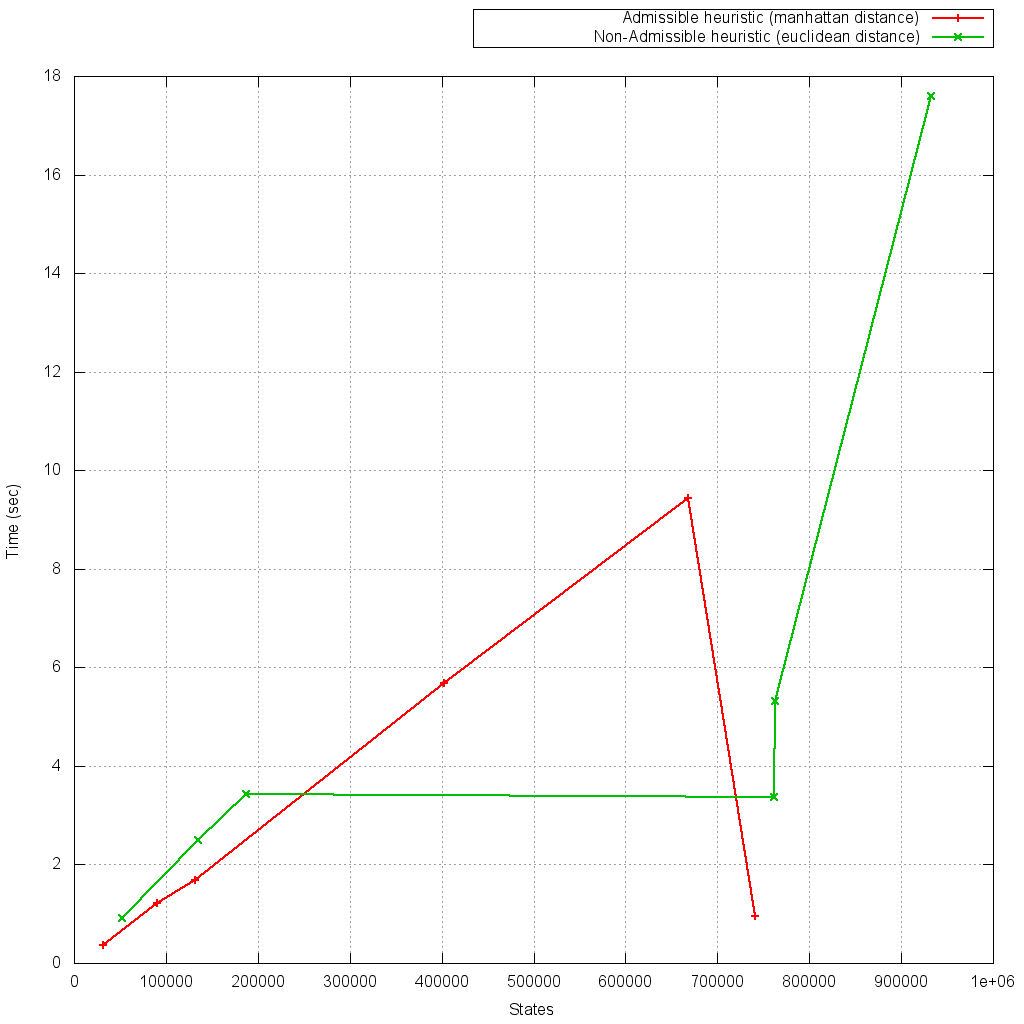
\includegraphics[scale=0.35]{../datafiles/graph.png}
\end{center}
\caption{Γραφική παράσταση για admissable και non-admissable heuristic }
\end{figure}

\section{Σχολιασμός αποτελεσμάτων}
Παρατηρούμε ότι και στα έξι testcase που δοκιμάσαμε η non-admissible ευριστική χρειάζεται να κατασκευάσει μεγαλύτερο δέντρο αναζήτησης, δηλαδή να παράγει περισσότερα states. Αυτό συμβαίνει επειδή η χρήση admissible ευριστικής αποτελεί απαραίτητη συνθήκη για να μπορέσει να βρεί ένα βέλτιστο μονοπάτι. Με τη χρήση non-admissible ευριστικής ο αλγόριθμος μπορεί να εξετάσει μονοπάτια που κανονικά δε θα έπρεπε, επειδή δεν είναι βέλτιστα, αλλά λόγω της υπερ-εκτίμησης ο αλγόριθμος δε το γνωρίζει αυτό και δε μπορεί να τα "κλαδέψει".
\end{document}
